\begin{frame}[fragile]{Exemplo de aritmética em Forth}

    \begin{tikzpicture}
        \node[anchor=west] at (1, 6.5) { \textbf{Expressão:} \code{forth}{1 2 3 + 4 * -} };
        \node[anchor=west] at (1, 5) { \textbf{Operação:} };
        \node[anchor=west] at (2, 4) { \textbf{Pilha:} };
        
        \draw[thick] (4.5, 0) to (6.5, 0);

        \pause

        \draw[-latex,color=blue] (3.23, 5.5) to (3.23, 6.25);

        \pause

        \draw (5, 0) rectangle (6, 1);
        \node at (5.5, 0.5) { \tt \textcolor{blue}{1} };

    \end{tikzpicture}

\end{frame}

\begin{frame}[fragile]{Exemplo de aritmética em Forth}

    \begin{tikzpicture}
        \node[anchor=west] at (1, 6.5) { \textbf{Expressão:} \code{forth}{1 2 3 + 4 * -} };
        \node[anchor=west] at (1, 5) { \textbf{Operação:} };
        \node[anchor=west] at (2, 4) { \textbf{Pilha:} };
        
        \draw[thick] (4.5, 0) to (6.5, 0);

        \draw[-latex,color=blue] (3.63, 5.5) to (3.63, 6.25);

        \draw (5, 0) rectangle (6, 1);
        \node at (5.5, 0.5) { \tt \textcolor{blue}{1} };

        \pause

        \draw (5, 1) rectangle (6, 2);
        \node at (5.5, 1.5) { \tt \textcolor{blue}{2} };
    \end{tikzpicture}

\end{frame}

\begin{frame}[fragile]{Exemplo de aritmética em Forth}

    \begin{tikzpicture}
        \node[anchor=west] at (1, 6.5) { \textbf{Expressão:} \code{forth}{1 2 3 + 4 * -} };
        \node[anchor=west] at (1, 5) { \textbf{Operação:} };
        \node[anchor=west] at (2, 4) { \textbf{Pilha:} };
        
        \draw[thick] (4.5, 0) to (6.5, 0);

        \draw[-latex,color=blue] (4.03, 5.5) to (4.03, 6.25);

        \draw (5, 0) rectangle (6, 1);
        \node at (5.5, 0.5) { \tt \textcolor{blue}{1} };

        \draw (5, 1) rectangle (6, 2);
        \node at (5.5, 1.5) { \tt \textcolor{blue}{2} };

        \pause

        \draw (5, 2) rectangle (6, 3);
        \node at (5.5, 2.5) { \tt \textcolor{blue}{3} };
    \end{tikzpicture}

\end{frame}

\begin{frame}[fragile]{Exemplo de aritmética em Forth}

    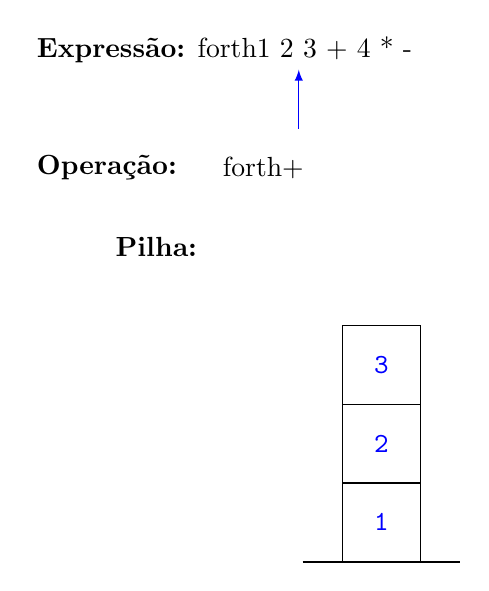
\begin{tikzpicture}
        \node[anchor=west] at (1, 6.5) { \textbf{Expressão:} \code{forth}{1 2 3 + 4 * -} };
        \node[anchor=west] at (1, 5) { \textbf{Operação:} };
        \node[anchor=west] at (2, 4) { \textbf{Pilha:} };
        
        \draw[thick] (4.5, 0) to (6.5, 0);

        \draw[-latex,color=blue] (4.45, 5.5) to (4.45, 6.25);

        \draw (5, 0) rectangle (6, 1);
        \node at (5.5, 0.5) { \tt \textcolor{blue}{1} };

        \draw (5, 1) rectangle (6, 2);
        \node at (5.5, 1.5) { \tt \textcolor{blue}{2} };

        \draw (5, 2) rectangle (6, 3);
        \node at (5.5, 2.5) { \tt \textcolor{blue}{3} };

        \pause

        \node at (4, 5) { \code{forth}{+} };

    \end{tikzpicture}

\end{frame}

\begin{frame}[fragile]{Exemplo de aritmética em Forth}

    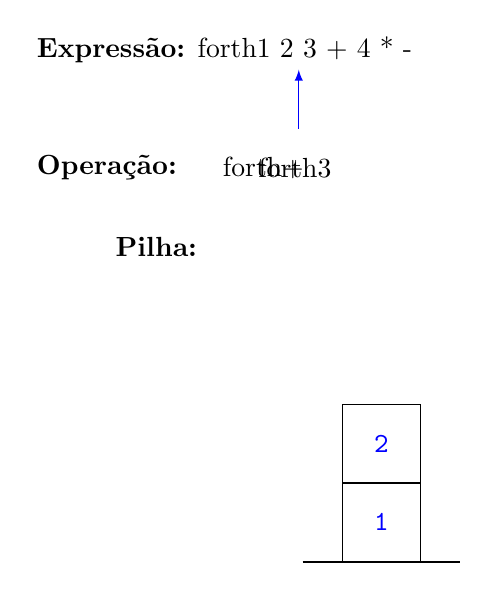
\begin{tikzpicture}
        \node[anchor=west] at (1, 6.5) { \textbf{Expressão:} \code{forth}{1 2 3 + 4 * -} };
        \node[anchor=west] at (1, 5) { \textbf{Operação:} };
        \node[anchor=west] at (2, 4) { \textbf{Pilha:} };
        
        \draw[thick] (4.5, 0) to (6.5, 0);

        \draw[-latex,color=blue] (4.45, 5.5) to (4.45, 6.25);

        \draw (5, 0) rectangle (6, 1);
        \node at (5.5, 0.5) { \tt \textcolor{blue}{1} };

        \draw (5, 1) rectangle (6, 2);
        \node at (5.5, 1.5) { \tt \textcolor{blue}{2} };

%        \draw (5, 2) rectangle (6, 3);
%        \node at (5.5, 2.5) { \tt \textcolor{blue}{3} };

        \node at (4, 5) { \code{forth}{+} };
        \node at (4.4, 5) { \code{forth}{3} };

    \end{tikzpicture}

\end{frame}

\begin{frame}[fragile]{Exemplo de aritmética em Forth}

    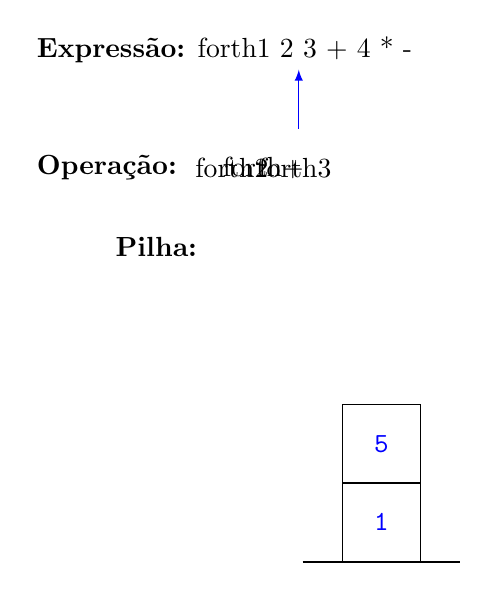
\begin{tikzpicture}
        \node[anchor=west] at (1, 6.5) { \textbf{Expressão:} \code{forth}{1 2 3 + 4 * -} };
        \node[anchor=west] at (1, 5) { \textbf{Operação:} };
        \node[anchor=west] at (2, 4) { \textbf{Pilha:} };
        
        \draw[thick] (4.5, 0) to (6.5, 0);

        \draw[-latex,color=blue] (4.45, 5.5) to (4.45, 6.25);

        \draw (5, 0) rectangle (6, 1);
        \node at (5.5, 0.5) { \tt \textcolor{blue}{1} };


%        \draw (5, 2) rectangle (6, 3);
%        \node at (5.5, 2.5) { \tt \textcolor{blue}{3} };

        \node at (4, 5) { \code{forth}{+} };
        \node at (4.4, 5) { \code{forth}{3} };
        \node at (3.6, 5) { \code{forth}{2} };

        \pause

        \draw (5, 1) rectangle (6, 2);
        \node at (5.5, 1.5) { \tt \textcolor{blue}{5} };

    \end{tikzpicture}

\end{frame}

\begin{frame}[fragile]{Exemplo de aritmética em Forth}

    \begin{tikzpicture}
        \node[anchor=west] at (1, 6.5) { \textbf{Expressão:} \code{forth}{1 2 3 + 4 * -} };
        \node[anchor=west] at (1, 5) { \textbf{Operação:} };
        \node[anchor=west] at (2, 4) { \textbf{Pilha:} };
        
        \draw[thick] (4.5, 0) to (6.5, 0);

        \draw[-latex,color=blue] (4.85, 5.5) to (4.85, 6.25);

        \draw (5, 0) rectangle (6, 1);
        \node at (5.5, 0.5) { \tt \textcolor{blue}{1} };

        \draw (5, 1) rectangle (6, 2);
        \node at (5.5, 1.5) { \tt \textcolor{blue}{5} };

        \pause

        \draw (5, 2) rectangle (6, 3);
        \node at (5.5, 2.5) { \tt \textcolor{blue}{4} };

%        \node at (4, 5) { \code{forth}{+} };
%        \node at (4.4, 5) { \code{forth}{3} };
%        \node at (3.6, 5) { \code{forth}{2} };

    \end{tikzpicture}

\end{frame}

\begin{frame}[fragile]{Exemplo de aritmética em Forth}

    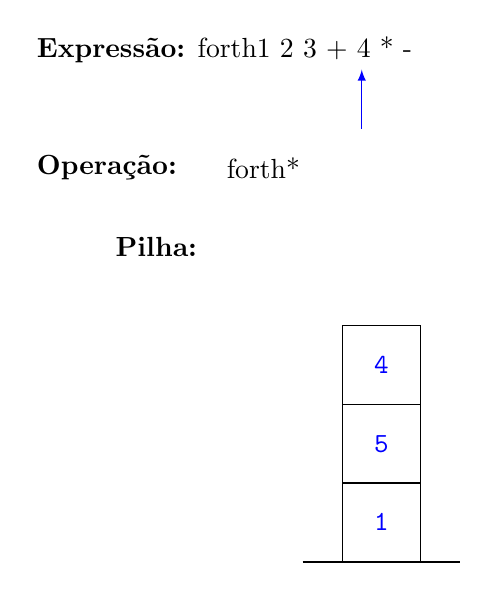
\begin{tikzpicture}
        \node[anchor=west] at (1, 6.5) { \textbf{Expressão:} \code{forth}{1 2 3 + 4 * -} };
        \node[anchor=west] at (1, 5) { \textbf{Operação:} };
        \node[anchor=west] at (2, 4) { \textbf{Pilha:} };
        
        \draw[thick] (4.5, 0) to (6.5, 0);

        \draw[-latex,color=blue] (5.25, 5.5) to (5.25, 6.25);

        \draw (5, 0) rectangle (6, 1);
        \node at (5.5, 0.5) { \tt \textcolor{blue}{1} };

        \draw (5, 1) rectangle (6, 2);
        \node at (5.5, 1.5) { \tt \textcolor{blue}{5} };

        \draw (5, 2) rectangle (6, 3);
        \node at (5.5, 2.5) { \tt \textcolor{blue}{4} };

        \pause
        \node at (4, 5) { \code{forth}{*} };
%        \node at (4.4, 5) { \code{forth}{3} };
%        \node at (3.6, 5) { \code{forth}{2} };

    \end{tikzpicture}

\end{frame}

\begin{frame}[fragile]{Exemplo de aritmética em Forth}

    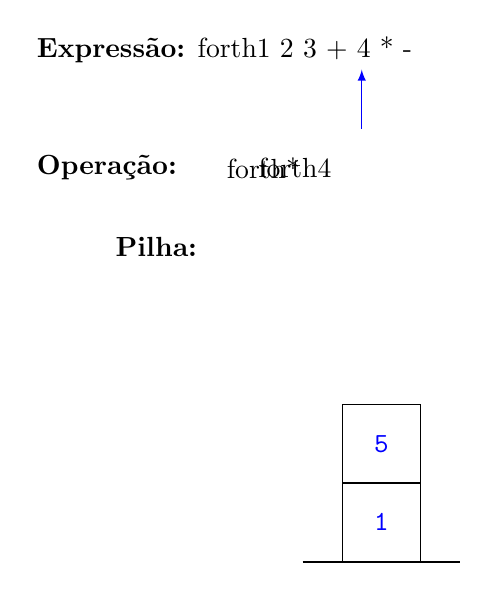
\begin{tikzpicture}
        \node[anchor=west] at (1, 6.5) { \textbf{Expressão:} \code{forth}{1 2 3 + 4 * -} };
        \node[anchor=west] at (1, 5) { \textbf{Operação:} };
        \node[anchor=west] at (2, 4) { \textbf{Pilha:} };
        
        \draw[thick] (4.5, 0) to (6.5, 0);

        \draw[-latex,color=blue] (5.25, 5.5) to (5.25, 6.25);

        \draw (5, 0) rectangle (6, 1);
        \node at (5.5, 0.5) { \tt \textcolor{blue}{1} };

        \draw (5, 1) rectangle (6, 2);
        \node at (5.5, 1.5) { \tt \textcolor{blue}{5} };

%        \draw (5, 2) rectangle (6, 3);
%        \node at (5.5, 2.5) { \tt \textcolor{blue}{4} };

        \node at (4, 5) { \code{forth}{*} };
        \node at (4.4, 5) { \code{forth}{4} };
%        \node at (3.6, 5) { \code{forth}{2} };

    \end{tikzpicture}

\end{frame}

\begin{frame}[fragile]{Exemplo de aritmética em Forth}

    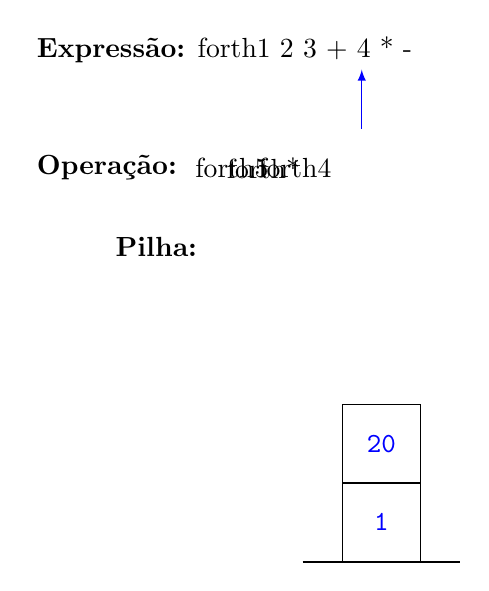
\begin{tikzpicture}
        \node[anchor=west] at (1, 6.5) { \textbf{Expressão:} \code{forth}{1 2 3 + 4 * -} };
        \node[anchor=west] at (1, 5) { \textbf{Operação:} };
        \node[anchor=west] at (2, 4) { \textbf{Pilha:} };
        
        \draw[thick] (4.5, 0) to (6.5, 0);

        \draw[-latex,color=blue] (5.25, 5.5) to (5.25, 6.25);

        \draw (5, 0) rectangle (6, 1);
        \node at (5.5, 0.5) { \tt \textcolor{blue}{1} };

        \node at (4, 5) { \code{forth}{*} };
        \node at (4.4, 5) { \code{forth}{4} };
        \node at (3.6, 5) { \code{forth}{5} };

        \pause

        \draw (5, 1) rectangle (6, 2);
        \node at (5.5, 1.5) { \tt \textcolor{blue}{20} };

    \end{tikzpicture}

\end{frame}

\begin{frame}[fragile]{Exemplo de aritmética em Forth}

    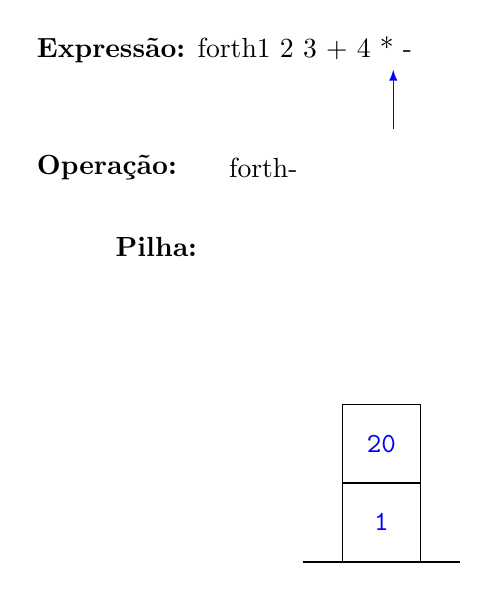
\begin{tikzpicture}
        \node[anchor=west] at (1, 6.5) { \textbf{Expressão:} \code{forth}{1 2 3 + 4 * -} };
        \node[anchor=west] at (1, 5) { \textbf{Operação:} };
        \node[anchor=west] at (2, 4) { \textbf{Pilha:} };
        
        \draw[thick] (4.5, 0) to (6.5, 0);

        \draw[-latex,color=blue] (5.65, 5.5) to (5.65, 6.25);

        \draw (5, 0) rectangle (6, 1);
        \node at (5.5, 0.5) { \tt \textcolor{blue}{1} };

        \draw (5, 1) rectangle (6, 2);
        \node at (5.5, 1.5) { \tt \textcolor{blue}{20} };

        \pause

        \node at (4, 5) { \code{forth}{-} };
        %\node at (4.4, 5) { \code{forth}{4} };
        %\node at (3.6, 5) { \code{forth}{5} };

    \end{tikzpicture}

\end{frame}

\begin{frame}[fragile]{Exemplo de aritmética em Forth}

    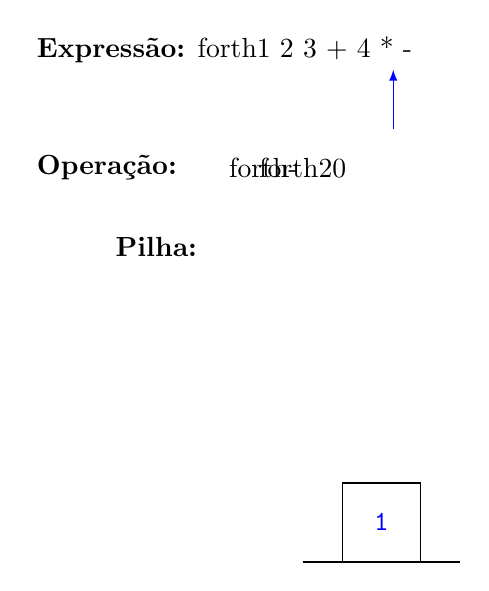
\begin{tikzpicture}
        \node[anchor=west] at (1, 6.5) { \textbf{Expressão:} \code{forth}{1 2 3 + 4 * -} };
        \node[anchor=west] at (1, 5) { \textbf{Operação:} };
        \node[anchor=west] at (2, 4) { \textbf{Pilha:} };
        
        \draw[thick] (4.5, 0) to (6.5, 0);

        \draw[-latex,color=blue] (5.65, 5.5) to (5.65, 6.25);

        \draw (5, 0) rectangle (6, 1);
        \node at (5.5, 0.5) { \tt \textcolor{blue}{1} };

        \node at (4, 5) { \code{forth}{-} };
        \node at (4.5, 5) { \code{forth}{20} };
        %\node at (3.6, 5) { \code{forth}{5} };

    \end{tikzpicture}

\end{frame}

\begin{frame}[fragile]{Exemplo de aritmética em Forth}

    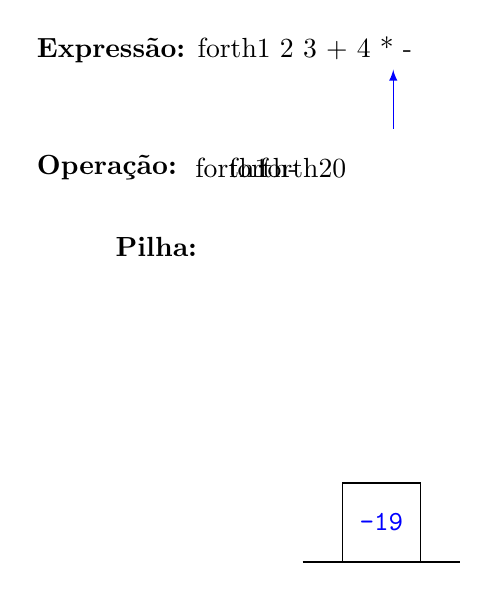
\begin{tikzpicture}
        \node[anchor=west] at (1, 6.5) { \textbf{Expressão:} \code{forth}{1 2 3 + 4 * -} };
        \node[anchor=west] at (1, 5) { \textbf{Operação:} };
        \node[anchor=west] at (2, 4) { \textbf{Pilha:} };
        
        \draw[thick] (4.5, 0) to (6.5, 0);

        \draw[-latex,color=blue] (5.65, 5.5) to (5.65, 6.25);

        \node at (4, 5) { \code{forth}{-} };
        \node at (4.5, 5) { \code{forth}{20} };
        \node at (3.6, 5) { \code{forth}{1} };

        \pause

        \draw (5, 0) rectangle (6, 1);
        \node at (5.5, 0.5) { \tt \textcolor{blue}{-19} };
    \end{tikzpicture}

\end{frame}

